\subsection{Presence of delay in our system}
We have delays in our system that are due to the sensor transmitting the information, the microcontroller processing that information and the actuator (piston) actually moving our mass damper. We have chosen that last source of delay as being the biggest one, with a frequency of \SI{50}{\hertz}, which induces delays of \SI{0.02}{\second}.\par
Some Bode and Nyquist plots showing delays are given at figures \ref{fig:bode-70}, \ref{fig:nyquist-70} and \ref{fig:nyquist-1}.\par
As can be seen, for a phase margin of \SI{70}{\degree}, the delays in our system do not bring instabilities. However, something strange is that a bigger phase margin seems to make our system less robust to delays, as can be seen on the two Nyquist plots given below. That is not how it should be, theoretically speaking. However, we have compared with the way you have designed your components, and do not see a difference.\par
Our lead compensator and gain have the same \og{}form\fg{} as the ones you have used. We have therefore included the Matlab script we have used to plot these figures in the mail we sent.
\begin{figure}[H]
    \centering
    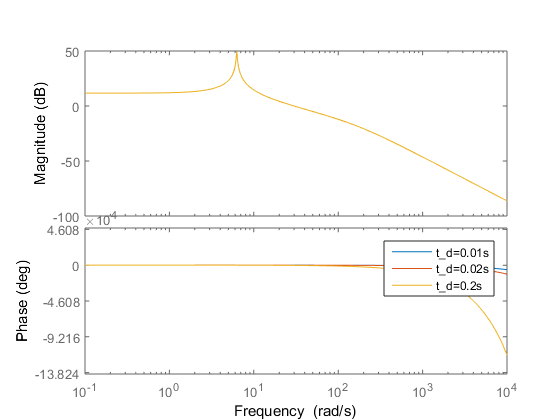
\includegraphics[width=0.8\textwidth]{resources/png/bode-70.png}
    \caption{Bode plots for various delays and a phase margin of 70 degrees.}
    \label{fig:bode-70}
\end{figure}
\begin{figure}[H]
    \centering
    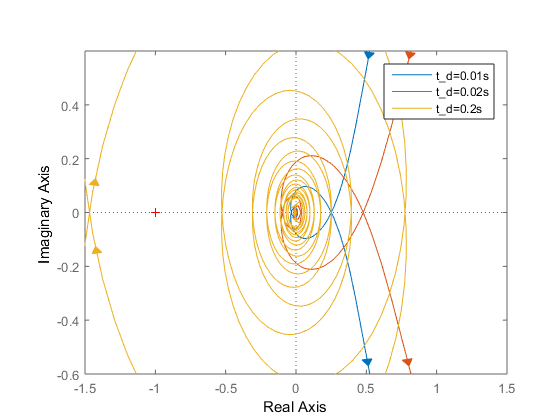
\includegraphics[width=0.8\textwidth]{resources/png/nyquist-70.png}
    \caption{Nyquist plots for various delays and a phase margin of 70 degrees.}
    \label{fig:nyquist-70}
\end{figure}
\begin{figure}[H]
    \centering
    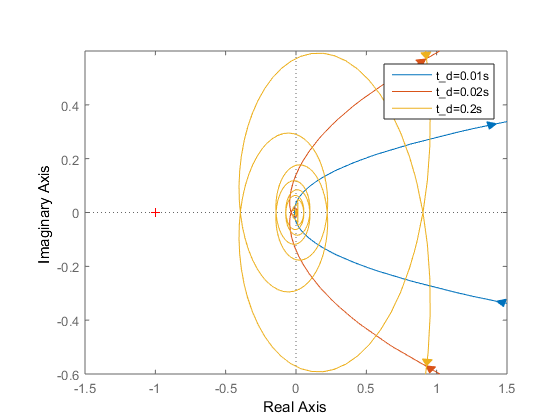
\includegraphics[width=0.8\textwidth]{resources/png/nyquist-1.png}
    \caption{Nyquist plots for various delays and a phase margin of 1 degree.}
    \label{fig:nyquist-1}
\end{figure}
